\section{Design}
The design describes *what* the structure of the system should be to fulfil the requirements.
Document the architecture and abstractions of the system.
Design develops those abstractions into realizable components.
Describe and sketch the *component models* of the game using a UML component diagram.
The component contracts in the system must be described in terms of pre- and post-conditions.
Furthermore, the different elements of the game and how they are connected must be described.

\subsection{UML Diagrams}
\subsubsection{Component}
\begin{figure}[H]
    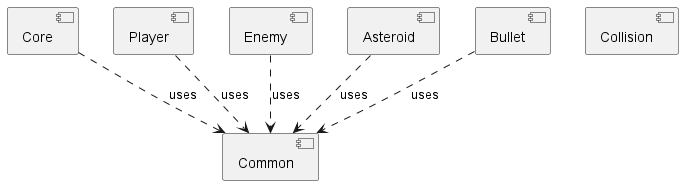
\includegraphics[width=\textwidth]{images/diagrams/component.png}
    \caption{A UML Component diagram over the project}
\end{figure}

\subsubsection{Class}
\begin{figure}[H]
    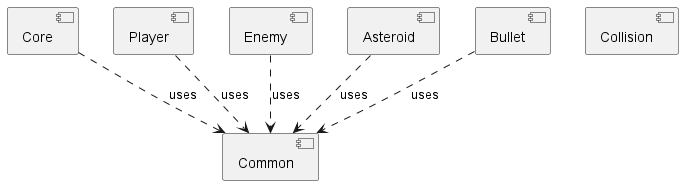
\includegraphics[width=\textwidth]{images/diagrams/component.png}
    \caption{A UML Class diagram over the project}
\end{figure}

\subsubsection{Sequence}
\begin{figure}[H]
    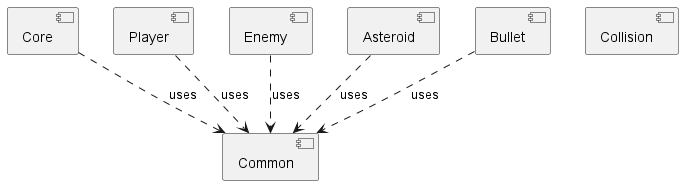
\includegraphics[width=\textwidth]{images/diagrams/component.png}
    \caption{A UML Sequence diagram over the project}
\end{figure}

\subsection{Component Contracts}
\subsubsection{IGamePluginService}
TEST
The IGamePluginService interface, is implemented by the plugins that are used to initialize entities handled by the different services.
This interface has two operations. One for starting the plugin and one for stopping the plugin.
\begin{figure}[H]
    \begin{center}
        \begin{tabulary}{1.0\textwidth}{lL}
            \toprule
            Operation:      & start(GameData gameData, World world) \\
            \midrule
            Description:     & Initializes the components' entities  \\
            \midrule
            Parameters:      & text                                  \\
            \midrule
            Preconditions:   & text                                  \\
            \midrule
            Postconditions:  & text                                  \\
            \bottomrule
        \end{tabulary}
    \end{center}
    \caption{Component contract over the functions of the IEntityProcessingService interface.}
\end{figure}

\begin{figure}[H]
    \begin{center}
        \begin{tabulary}{1.0\textwidth}{lL}
            \toprule
            Operation:      & stop(GameData gameData, World world)                       \\
            \midrule
            Description:     & Cleans up entities that were initialized by the components \\
            \midrule
            Parameters:      & text                                                       \\
            \midrule
            Preconditions:   & text                                                       \\
            \midrule
            Postconditions:  & text                                                       \\
            \bottomrule
        \end{tabulary}
    \end{center}
    \caption{Component contract over the functions of the IEntityProcessingService interface.}
\end{figure}

\subsubsection{IEntityProcessingService}
The IEntityProcessingService interface is implemented by components' services, so that they can process and handle game
logic every frame.
\begin{figure}[H]
    \begin{center}
        \begin{tabulary}{1.0\textwidth}{lL}
            \toprule
            Operation:      & process(GameData gameData, World world) \\
            \midrule
            Description:     & Processes game logic                    \\
            \midrule
            Parameters:      & text                                    \\
            \midrule
            Preconditions:   & text                                    \\
            \midrule
            Postconditions:  & text                                    \\
            \bottomrule
        \end{tabulary}
    \end{center}
    \caption{Component contract over the functions of the IEntityProcessingService interface.}
\end{figure}

\subsubsection{IPostEntityProcessingService}
The IEntityProcessingService interface is, like the IEntityProcessingService, implemented by components' services, so that they can process and handle game
logic every frame. The IPostEntityService, however, always processes after each IEntityProcessingService has finished processing.
\begin{figure}[H]
    \begin{center}
        \begin{tabulary}{1.0\textwidth}{lL}
            \toprule
            Operation:      & process(GameData gameData, World world) \\
            \midrule
            Description:     & Processes game logic.                   \\
            \midrule
            Parameters:      & text                                    \\
            \midrule
            Preconditions:   & text                                    \\
            \midrule
            Postconditions:  & text                                    \\
            \bottomrule
        \end{tabulary}
    \end{center}
    \caption{Caption}
\end{figure}

\subsubsection{IBulletFactory}
The IBulletFactory is an interface implemented by classes that need implementation logic specifically for spawning bullets.
\begin{figure}[H]
    \begin{center}
        \begin{tabulary}{1.0\textwidth}{lL}
            \toprule
            Operation:      & create(Entity sourceEntity, GameData gameData)                                       \\
            \midrule
            Description:     & Creates the bulletfactory, sets the source entity and returns a new bullet to spawn. \\
            \midrule
            Parameters:      & text                                                                                 \\
            \midrule
            Preconditions:   & text                                                                                 \\
            \midrule
            Postconditions:  & text                                                                                 \\
            \bottomrule
        \end{tabulary}
    \end{center}
    \caption{Caption}
\end{figure}

\subsubsection{EntityPart}
The EntityPart is an interface implemented by the different parts that can be attached to an entity to extend the logic of said entity.
\begin{figure}[H]
    \begin{center}
        \begin{tabulary}{1.0\textwidth}{lL}
            \toprule
            Operation:      & process(GameData gameData, Entity entity)                                 \\
            \midrule
            Description:     & Processes game logic to do with the entity that said part is attached to. \\
            \midrule
            Parameters:      & text                                                                      \\
            \midrule
            Preconditions:   & text                                                                      \\
            \midrule
            Postconditions:  & text                                                                      \\
            \bottomrule
        \end{tabulary}
    \end{center}
    \caption{Caption}
\end{figure}


\subsection{Elements of the game}
Describe the different elements of the game and how they are connected.
Maybe do this together with component diagram?